\section{Diskussion}
Im Rahmen dieser Arbeit wurde ein System zum klassifizieren von Sprachaufnahmen implementiert. Das Programm unterscheidet zwischen Französisch, Deutsch, und Englisch. Mit Deep Learning hat das Programm selbst gelernt die Sprache von kurzen Aufnahmen zu erkennen. Anstatt rohe Schallwellen zu verarbeiten wurden in Echtzeit berechnete Spektrogramme verwendet. Die Spektrogramme konnten mit Bilderkennungsmethoden erfolgreich eingeordnet werden. Ein hybrides Modell aus CNN und RNN besass die höchste Genauigkeit. Die Trainingsdaten wurden wegen fehlenden maßgeschneiderten Datensets aus verschiednen Quellen selbst kompiliert. Es wurde mit Daten von Voxforge und Youtube trainiert um mit Daten aus der Librivox Hörbuchdatenbank getestet zu werden. Die hohe Korrektheit aller Modelle bestätigt, dass tiefe neuronale Netze eine angemessene Methode für Sprachidentifikation sind.
\\ \\
Der Vergleich der Resultate mit anderen Arbeiten ist nur mit Vorsicht möglich. Der wichtigste Unterschied ist, dass andere Daten verwendet werden und dementsprechend nur andere Resultate entstehen können. Glücklicherweise sind Arbeiten zu Automatischer Sprachidentifikation im Internet jedoch frei erhältlich, denn das Problem ist in der Informatik recht jung. Erst in den 70'er Jahren wurde man für das weiterleiten von Telefonanrufen auf das Thema aufmerksam. Eine lange Zeit galt, dass die bessten Systeme diejenigen waren, die die fortgeschrittensten sprachlichen Merkmale berechneten. Der Nachteil an diesen Systemen ist, dass die Erweiterung auf andere Sprachen mit einem grossem Aufwand verbunden ist. \parencite{history}
\\
Erst mit dem Aufkommen von Deep Learning als konkurrenzfähige Methode im letzen Jahrzehnt kamen wieder Systeme mit weniger Preprocessing auf \parencite{chollet}. 2009 erreichte Grégoire Montavon mit Deep Learning für 3 Sprachen auf dem Voxforge Datenset eine Genauigkeit von $80.1\%$ \parencite{montavon}. Das Voxforge Datenset hat sich seither verändert. Es kann angenommen werden, dass die hier vorgestellten Modelle, sein System deutlich übertreffen, da ähnliche Arbeiten dass getestet haben \parencite{iLID}. 2016 wurde mit einem sehr ähnlichen Modell wie das CNN Modell dieser Arbeit Genauigkeiten von 93\% und 85\% für 2 Sprachen respektive 4 Sprachen gemessen \parencite{iLID}. Hrayr et al. \parencite{yerevann} stellen im selben Jahr ein CRNN Modell für einen Wettbewerb vor, dass zwischen 176 Sprachen mit 99.67\% Genauigkeit differenzieren kann. Ein weiteres CRNN Modell von Bartz et al. \parencite{crnn} erreicht 2017 91\% bei der Unterscheidung von vier Sprachen.
\\
Die in dieser Arbeit vorgestellten System leisten vergleichbare Genaugigkeiten wie die genannten Modelle. 95\% ist eine höchst zufriedenstellende Genauigkeit unter anbetracht das das Youtube Datenset nicht fehlerfrei ist. Das Datenset wurde bekanntlich nicht manuell gesäubert. Es können dementsprechend Aufnahmen ohne Sprache oder mit fremdsprachigen Interviews enthalten sein. Der Anteil von fehlerhaften Aufnahmen ist jedoch wahrscheinlich klein. 
Der Fall auf 80\% Genauigkeit beim Librivox Datenset ist normal. Das Modell ist selbstverständlich für die Youtube und Voxforge Daten optimiert und nicht für Hörbücher. Die Librivox Daten haben zum Beispiel unterschiedliche Hintergrundgeräusche und Aufnahmeprotokolle. 80\% bleibt in jedem Fall ein erfreuliches Resultat. Ein Zufallsgenerator würde im Kontrast nur 33\% erreichen. Es kann also aus dem Resultat abgelesen werden, dass das Modell angemessen generalisiert. 
\\ \\
Bis jetzt wurde das Modell nur an öffentlich verfügbaren Daten ausgewertet wo klar war welche Sprache gesprochen wurde. In der Realität soll das Modell aber helfen die Sprache von unbekannten Aufnahmen zu erkennen. In anderen Worten soll das Modell in der Praxis angewendet werden. Dafür wurde ein Interface programmiert wo Benutzer sich selbst Aufnehmen und das Modell damit abfragen können. Das Interface ist in Form einer Webseite auf den Schulservern frei verfügbar (Die meisten Mobilgeräte und Computer sind kompatibel):
\begin{figure}[hbt]
	\centering
		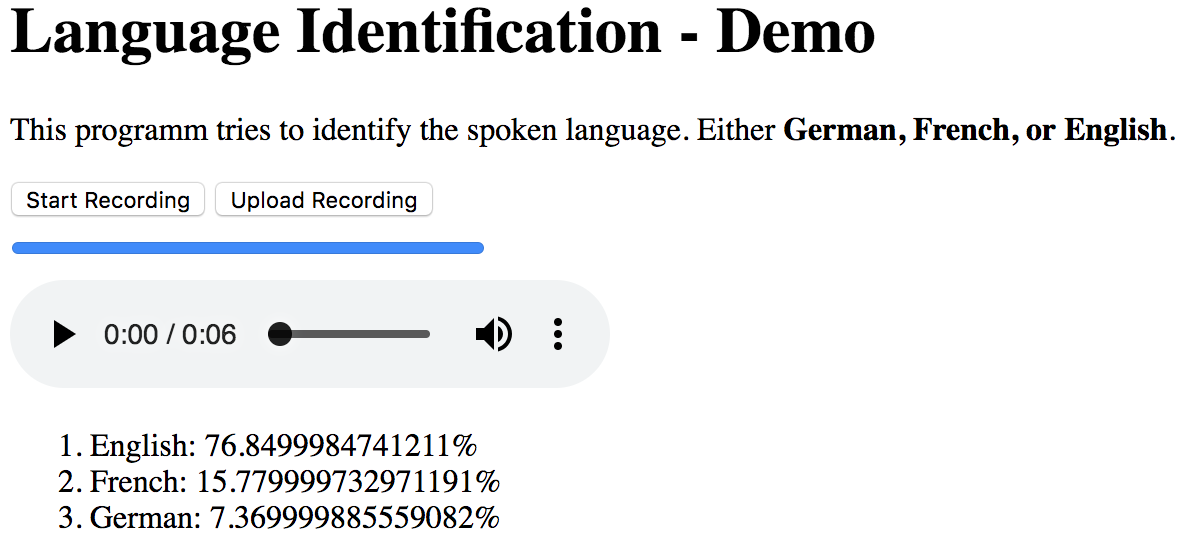
\includegraphics[width=0.6\textwidth]{assets/interface.png}
	\caption{Interface Schnappschuss}
	\label{img:interface}
\end{figure}
Die Umgebung bei Smartphone Aufnahmen ist erneut eine andere wie die von Voxforge und YouTube. Die Genauigkeit die dort erreicht wird ist eine weitere Art die Generalisierbarkeit des Modells zu messen. Aus Neugier wurde ein sehr kleines Datenset aus Aufnahmen von Verwandten und Freunden zusammengestellt. Es wurde darauf geachtet, dass die Sprache deutlich verständlich ist. Insgesamt sind es nur 70 ungleichmässig verteilte Aufnahmen. Die Resultate daraus sind wegen der kleinen Anzahl und Varianz kaum signifikant. Das Programm entdeckt in 70\% der Fälle die richtige Sprache. 

\parencite{history}
1. Gut -> Vergleich
	- iLID 92.9\%
	- crnn 91\%, inception 95\%
2. What you truly want -> Webserver
3. guru 
4. it's bad -> improving
5. data augmentation, more power
more data doesn't help, -> better data or model undercuts
fine tuning
more validation data


\subsection{Zuverlässigkeit}
\subsection{Erweiterung}
